\documentclass{article}
\usepackage[utf8]{inputenc}
\usepackage[T5]{fontenc}
\usepackage[fontsize=13px]{scrextend}
\usepackage[paperheight=29.7cm,paperwidth=21cm,right=2cm,left=3cm,top=2cm,bottom=2.5cm]{geometry}
\usepackage{mathptmx}
\usepackage{graphicx}
\usepackage{float}
\usepackage{tikz}
\usepackage{indentfirst} %thu vien thut dau dong
\usepackage{amsmath}
\usepackage{amsfonts}
\usepackage{amssymb}
\usepackage{enumitem}
\usepackage{subcaption}
\usetikzlibrary{calc}
\renewcommand{\baselinestretch}{1.2} %gianx dongf la 1.2
\setlength{\parskip}{6pt}
\setlength{\parindent}{1cm}
\usepackage{titlesec} %thu vien set up cac kieu chu
\titlespacing*{\section}{0pt}{0pt}{30pt}  %heading1
\titleformat*{\section}{\fontsize{16pt}{0pt}\selectfont \bfseries\centering}

\titlespacing*{\subsection}{0pt}{10pt}{0pt} %heading2
\titleformat*{\subsection}{\fontsize{14pt}{0pt}\selectfont \bfseries}

\titlespacing*{\subsection}{0pt}{10pt}{0pt} %heading 3
\titleformat*{\subsection}{\fontsize{13pt}{0pt}\selectfont \bfseries\itshape}

\titlespacing*{\paragraph}{0pt}{0pt}{30pt} %heading 4
\titleformat*{\paragraph}{\fontsize{16pt}{0pt}\selectfont \bfseries\itshape}

\begin{document}
\begin{titlepage}
    \begin{tikzpicture}[overlay,remember picture]
        \draw[line width=3pt]
        ($(current page.north west)+(3.0cm,-2.0cm) $)
        rectangle
        ($(current page.south east)+(-2.0cm,2.5cm)$);
        \draw[line width=1pt]
        ($(current page.north west)+(3.1cm,-2.1cm) $)
        rectangle
        ($(current page.south east)+(-2.1cm,2.6cm)$);
    \end{tikzpicture}

\begin{center}
    \vspace{-10pt} ĐẠI HỌC BÁCH KHOA HÀ NỘI\\
    \textbf{\fontsize{16pt}{0pt}\selectfont VIỆN ĐIỆN}
    \vspace{0.5cm}
    \begin{figure}[H]
        \centering
        
\includegraphics[width=2cm,height=3cm]{image/logo.png}
    \end{figure}


    \vspace{1cm}
    \fontsize{24pt}{0pt}\selectfont ĐỒ ÁN I\\
\end{center}
\hspace{15pt} \textbf{\fontsize{14pt}{0pt}\selectfont Đề tài:\\}
\begin{center}
    \textbf{\fontsize{20pt}{0pt}\selectfont MẠCH PHẦN CỨNG VÀ\\}
    \textbf{\fontsize{20pt}{0pt}\selectfont TRUYỀN THÔNG RF CHO HỆ THỐNG \\}
    \textbf{\fontsize{20pt}{0pt}\selectfont THU THẬP DỮ LIỆU PIR \\}
\end{center}
\vspace{1cm}
\begin{tabular}{l l}
    \hspace{15pt}
    \fontsize{14pt}{0pt}\selectfont Nhóm sinh viên: & \fontsize{20pt}{0pt}\selectfont Nguyễn Thái Sơn 20212951\\
    &\fontsize{20pt}{0pt}\selectfont Nguyễn Văn Mừng 20212894\\
    \hspace{15pt}
    \fontsize{14pt}{0pt}\selectfont Giảng viên hướng dẫn: & \fontsize{20pt}{0pt}\selectfont PGS.TS Nguyễn Quốc Cường  \\
   

\end{tabular}

\hspace{9cm} \textit{\textbf{\fontsize{14pt}{0pt}\selectfont Chữ kí của GVHD\\}}
\vspace{3cm}
\begin{center}
    \fontsize{14pt}{0pt}\selectfont Hà Nội, 6-2024
\end{center}
\end{titlepage}
\cleardoublepage
\section*{LỜI NÓI ĐẦU}
\thispagestyle{empty}

Trong thời đại số hóa ngày nay, sự phát triển của công nghệ đã mở ra không gian rộng lớn cho các ứng dụng nhúng và thiết bị thông minh, với mục đích tối ưu hóa các quy trình và tăng cường tiện ích trong cuộc sống hàng ngày. Trong ngữ cảnh này, cảm biến hồng ngoại chủ động (PIR - Passive Infrared Sensor) đã nổi lên như một công nghệ vô cùng quan trọng và có ứng dụng rộng rãi trong nhiều lĩnh vực Smart Home.

PIR không chỉ là một thiết bị cảm biến thông thường mà còn là một công cụ linh hoạt và hiệu quả trong việc phát hiện chuyển động dựa trên các dòng nhiệt hồng ngoại. Nhờ tính nhạy cao và khả năng hoạt động đáng tin cậy, PIR giúp giảm tải công việc của con người trong các quy trình điều khiển tự động, đồng thời mang lại sự tiện lợi và an toàn cho người dùng.

Trong báo cáo này, chúng tôi đặt ra mục tiêu xây dựng một hệ thống bao gồm mạch cứng và phần mềm để thu phát, lưu trữ và thao tác trên dữ liệu từ cảm biến hồng ngoại chủ động (PIR). Mạch cứng PIR Array được thiết kế với 5 cảm biến PIR, có khả năng thu thập tín hiệu hồng ngoại từ môi trường xung quanh và trả về giá trị ADC trong khoảng từ 0 đến 4095. Đồng thời, hệ thống phần mềm được phát triển để đọc và lưu trữ dữ liệu từ PIR Array, cung cấp công cụ để thu thập dữ liệu và thực hiện việc gán nhãn. Mục tiêu của đề tài là nghiên cứu và triển khai giải pháp toàn diện để xử lý và phân tích dữ liệu từ PIR Array, nhằm hỗ trợ các ứng dụng trong các lĩnh vực nhúng và các hệ thống thông minh. Báo cáo sẽ tập trung vào phân tích cấu trúc, hoạt động của hệ thống cảm biến PIR và các kỹ thuật xử lý dữ liệu để áp dụng vào các ứng dụng thực tế.

\vspace{2cm}

\hspace*{\fill}\textit{\textbf{\fontsize{14pt}{0pt}\selectfont Team PIR HARDWARE}}

\cleardoublepage
\addtocontents{toc}{\protect\thispagestyle{empty}}
\tableofcontents %tao muc luc tu dong
\thispagestyle{empty}

\cleardoublepage
%\addtocontentsline{toc}{section}{\numberline{}Giới thiệu chung}
\pagenumbering{arabic}
\section*{Chương 1.Giới thiệu chung}
\addcontentsline{toc}{section}{\numberline{}Chương 1.Giới thiệu chung}
\setcounter{section}{1}
Trong thời đại số hóa hiện nay, công nghệ nhúng và cảm biến thông minh đang ngày càng phát triển mạnh mẽ, đem lại nhiều lợi ích trong các ứng dụng công nghiệp và Smart Home. Cảm biến hồng ngoại chủ động (PIR) với tính nhạy cao và giá thành hợp lý được coi là một công nghệ quan trọng trong việc phát hiện chuyển động. Dự án này nhằm xây dựng một hệ thống bao gồm mạch cứng PIR Array và phần mềm để thu phát, lưu trữ và xử lý dữ liệu từ các cảm biến PIR. Mục tiêu là nghiên cứu và triển khai giải pháp nhằm hỗ trợ các ứng dụng thực tế, đặc biệt là trong lĩnh vực nhúng và hệ thống Smart Home.
\subsection{Lý do chọn đề tài }
Hiện nay, nhu cầu về các thiết bị nhúng cũng như cảm biến thông minh ngày càng lớn do khả năng ứng dụng rộng rãi của nó: trong các quá trình điều khiển công nghiệp, trên xe cộ cũng như các hệ thống Smart Home. Một cảm biến thông minh là cảm biến có thể đo đạc được các chỉ số của môi trường xung quanh để tự đưa ra những quyết định điều khiển đúng đắn, giúp giảm tải sự can thiệp của con người và đem đến các trải nghiệm tiện lợi. 

PIR (Passive infrared sensor) là cảm biến hồng ngoại phát có thể phát hiện chuyển động của vật thể trong 1 phạm vi nhất định. Với giá thành rẻ và tính nhỏ gọn, việc áp dụng PIR để làm cảm biến thông minh định vị được vị trí vật thể sẽ có tính ứng dụng rất cao trong các hệ thống nhúng nói chung và thiết bị Smart Home nói riêng. 
\subsection{Mục đích của đề tài}
Mục tiêu của đề tài này là đưa ra được một hệ thống mạch cứng và phần mềm để thu phát, lưu trữ và thao tác trên dữ liệu PIR bao gồm: 
\begin{itemize}
    \item Một mạch cứng PIR Array bao gồm 5 PIR, thu tín hiệu hồng ngoại của môi trường xung quanh và trả về giá trị ADC trong khoảng từ 0 đến 4095
    \item Hệ thống phần mềm để đọc và lưu trữ dữ liệu từ PIR Array, đồng thời cung cấp công cụ để lấy dữ liệu và gán nhãn. 
\end{itemize}
\subsection{Mục tiêu cụ thể}
Các thành phần cụ thể của hệ thống cần đạt được bao gồm: 
\begin{itemize}
    \item Mạch cứng PIR Array. 
    \item Vi điều khiển để đọc giá trị mạch cứng theo thời gian thực và gửi dữ liệu giá trị đó đi. 
    \item Server với Database để nhận và lưu trữ dữ liệu từ vi điều khiển, đồng thời cung cấp các API để lấy các dữ liệu
    \item Ứng dụng Desktop để: điều khiển bật tắt quá trình ghi dữ liệu, quay video tương ứng của môi trường ghi, đồng thời gán nhãn cho dữ liệu. 
\end{itemize}
Yêu cầu về dữ liệu được ghi: Là dữ liệu của cả 5 con PIR trong PIR Array, được ghi theo thời gian thực với chu kì 10ms. Mỗi giây sẽ gửi server một gói dữ liệu bao gồm 500 giá trị của 5  PIR. 
\cleardoublepage
\section*{Chương 2.Mô tả bài toán}
\addcontentsline{toc}{section}{\numberline{}Chương 2.Mô tả bài toán}
\setcounter{section}{2}
\setcounter{subsection}{0}
Đề tài này tập trung phát triển hệ thống cảm biến hồng ngoại chủ động (PIR) gồm mạch cứng, vi điều khiển ESP32, server và phần mềm quản lý. Mạch cứng với 5 PIR thu thập tín hiệu và trả về giá trị ADC từ 0-4095. Vi điều khiển đọc và gửi dữ liệu qua Wi-Fi mỗi 10ms. Server sử dụng C++ và SQLite để lưu trữ và xử lý dữ liệu, trong khi ứng dụng desktop được phát triển bằng NodeJS để quản lý, trực quan hóa và gán nhãn dữ liệu. Hệ thống đảm bảo thu thập dữ liệu ổn định, xử lý nhanh chóng và dễ mở rộng.
\subsection{Vấn đề cần giải quyết}
Các vấn đề cần giải quyết ở từng thành phần bao gồm: 
\subsubsection{Mạch cứng PIR Array }
PIR Array: gồm 5 PIR cùng cách mạch khuếch đại, chạy liên tục trong thời gian dài, giá trị voltage trả về phải nằm trong khoảng từ 0 – 4095.
\subsubsection{Vi điều khiển}
\begin{itemize}
    \item Phải chạy song song được 2 tác vụ là đọc dữ liệu từ PIR Array và đóng gói, gửi dữ liệu tới Server. 
    \item Dữ liệu ghi phải đều, đúng chu kì 10ms
    \item Vi điều khiển gửi dữ liệu qua đường truyền không dây, cụ thể với dự án này là qua Wifi. 
\end{itemize}
\subsubsection{Server và Database.}
\begin{itemize}
    \item Nhỏ gọn về dung lượng. 
    \item Xử lý dữ liệu nhanh với khả năng chịu tải đủ tốt phù hợp với chu kì gửi 1 giây / lần cùng lượng dữ liệu lớn được gửi đến. 
    \item Đưa ra giao thức phù hợp, dễ sử dụng để gửi và đọc dữ liệu
    \item Chạy ổn định trong thời gian dài mà không xảy ra sập, ngắt server. 
    \item Có tính bảo trì, mở rộng cao. 
\end{itemize}
\subsubsection{Phần mềm quản lý }
\begin{itemize}
    \item Điều khiển ghi dữ liệu cùng quay video theo thời gian thực. 
    \item Trực quan hóa dữ liệu bằng đồ thị theo thời gian thực. 
    \item Hỗ trợ gán nhãn, xuất ra file CSV. 
\end{itemize}
\subsection{Lựa chọn phương pháp }
\begin{figure}[H]
    \centering
    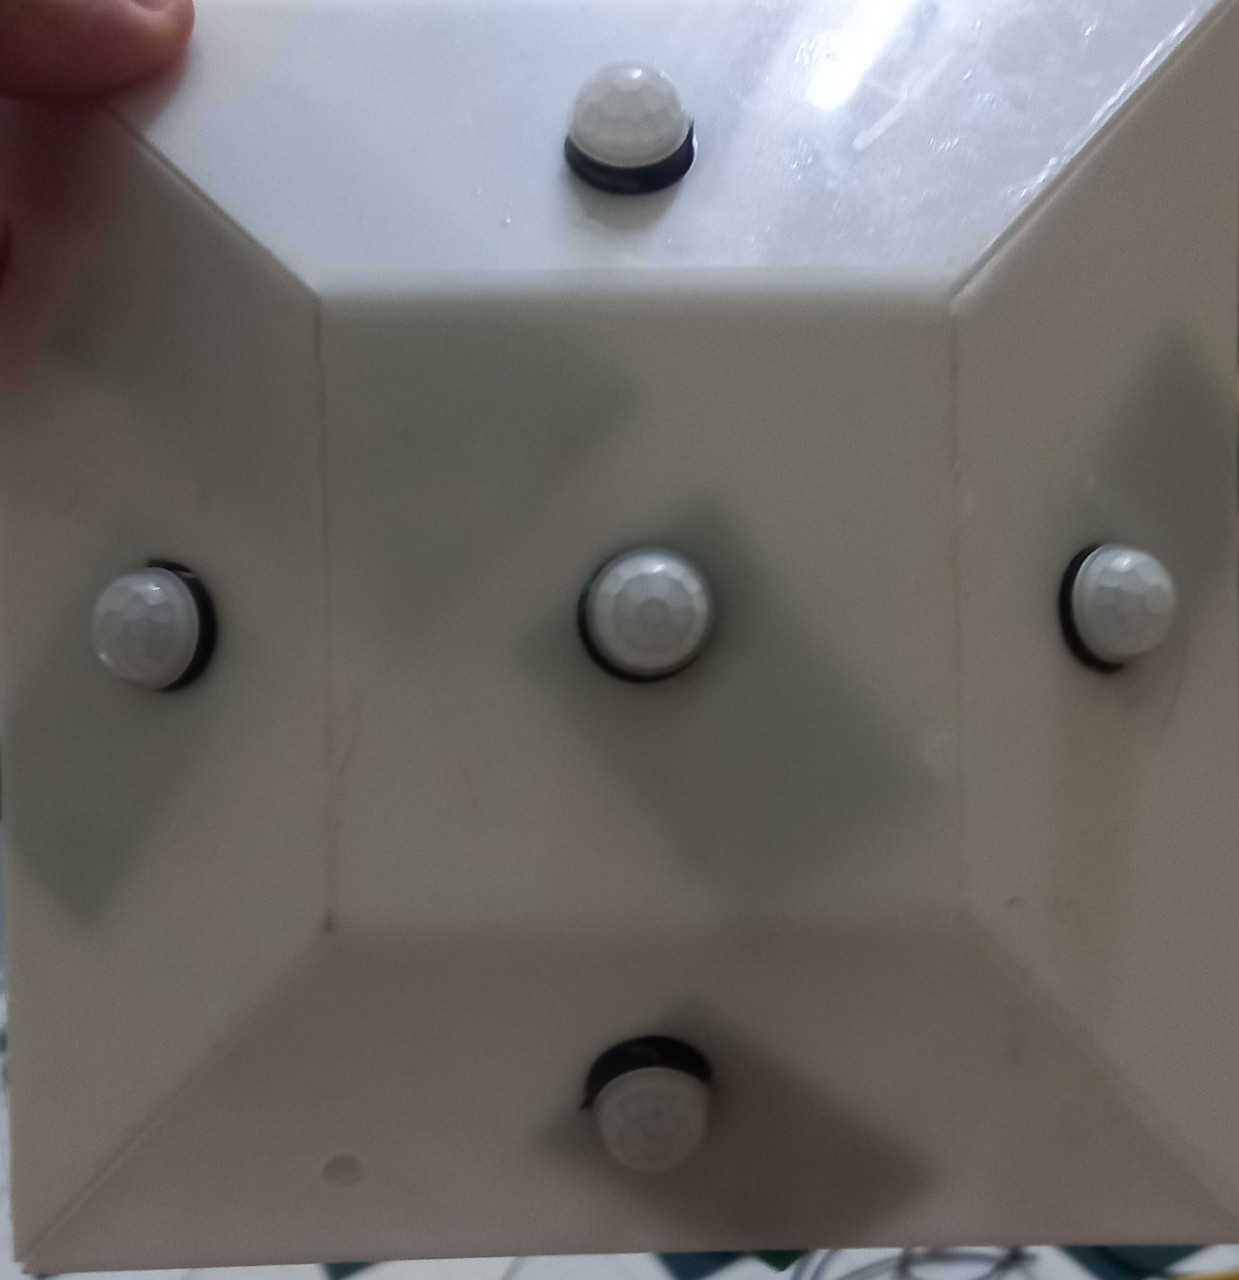
\includegraphics[width=7cm,height=7cm]{image/anh_pir.jpg}
    \caption{Mạch cứng PIR} \label{EV}
\end{figure}
Định nghĩa: Cảm biến PIR là một mạch cảm biến điện tử cảm ứng ánh sáng hồng ngoại phát ra từ các vật thể trong trường nhìn của nó. Về mặt kỹ thuật, PIR là một cảm biến nhiệt điện có thể phát hiện các mức bức xạ hồng ngoại kháy nhau. PIR có thể phát hiện chuyển động của người, động vật trong phạm vi yêu cầu một cách thụ động, bởi yêu cầu của thông số kỹ thuật cụ thể  
\begin{figure}[H]
    \centering
    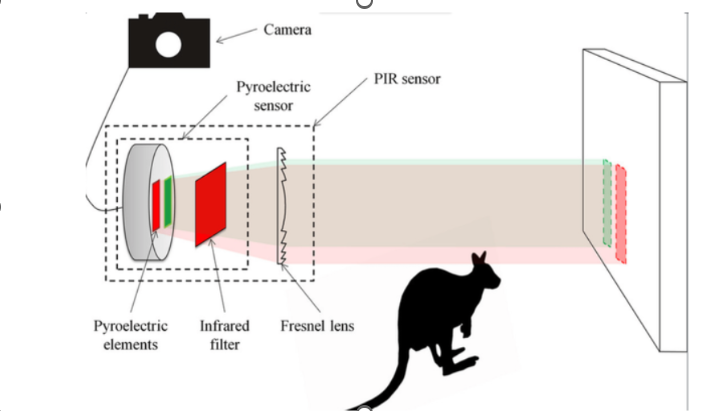
\includegraphics[width=10cm,height=5cm]{image/anh2.png}
    \caption{Cảm biến hồng ngoại PIR Sensor} \label{EV}
\end{figure}
Khi nguồn phát chuyển động vào vùng phát hiện (vùng có cả 2 kính hội tụ) thì tín hiệu sin nhảy mức cho điện áp ra. Sau đó, nguồn chuyển động khỏi vùng phát hiện, mạch trễ vẫn sẽ lưu giữ tín hiệu sau đó mới mất hẳn
\begin{figure}[H]
    \centering
    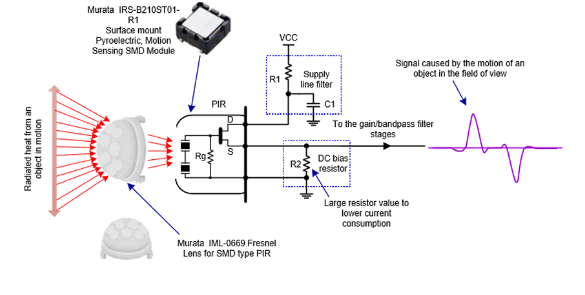
\includegraphics[width=10cm,height=5cm]{image/anh_3.png}
    \caption{Nguyên lý hoạt động} \label{EV}
\end{figure}
\subsubsection{Vi điều khiển}
Sử dụng vi điều khiển ESP32 với ADC độ phân giải 12 bit, dải giá trị đầu ra 0-4095. 
ESP32 là một vi điều khiển mạnh mẽ và linh hoạt, thường được sử dụng trong các ứng dụng IoT và các dự án nhúng nhờ khả năng kết nối Wi-Fi và Bluetooth tích hợp sẵn. 
ADC (Analog to Digital Converter) trên ESP32 cho phép chuyển đổi tín hiệu analog sang tín hiệu số với độ phân giải 12 bit. Điều này có nghĩa là tín hiệu analog được chuyển đổi thành một giá trị số trong khoảng từ 0 đến 4095. 

Ví dụ, nếu  kết nối một cảm biến nhiệt độ analog vào ESP32, tín hiệu analog từ cảm biến có thể được chuyển đổi thành các giá trị số để vi điều khiển có thể xử lý. 

ADC trên ESP32 có một số kênh, cho phép đọc tín hiệu từ nhiều nguồn khác nhau. Các kênh ADC này có thể được cấu hình và sử dụng một cách độc lập. 

Một số điểm cần lưu ý khi sử dụng ADC trên ESP32: 
\begin{itemize}
    \item \textbf{Độ phân giải:} Với độ phân giải 12 bit, có thể nhận được 4096 mức giá trị khác nhau từ 0 đến 4095. 
    \item \textbf{Điện áp tham chiếu:} Điện áp tham chiếu mặc định cho ADC trên ESP32 là từ 0V đến 3.3V. Điều này có nghĩa là giá trị 0 tương ứng với 0V và giá trị 4095 tương ứng với 3.3V. 
    \item \textbf{Tốc độ lấy mẫu:} ESP32 có thể lấy mẫu tín hiệu analog ở tốc độ cao, phù hợp cho các ứng dụng yêu cầu cập nhật dữ liệu nhanh. 
    \item \textbf{Hiệu chỉnh:} ADC trên ESP32 có thể cần được hiệu chỉnh để đảm bảo độ chính xác, do có thể có sai số do đặc điểm phần cứng và môi trường. 
\end{itemize}
\subsubsection{Server và Database }
\textbf{Về giao thức:}
\begin{itemize}
    \item Giao thức tầng transport sử dụng TCP/IP, tầng application sử dụng HTTP. 
    \item Ngôn ngữ là C++, xử lý giao thức sử dụng C++ Socket
\end{itemize}
Phát triển một HTTP Module, tức là một thư viện HTTP Server, để xử lý giao thức HTTP.

\textbf{Mô hình MVC:}
\begin{itemize}
    \item Model: Chứa các hàm ORM cho SQLite Database
    \item View: là các trang HTML đơn giản cung cấp thông tin về Server, đồng thời là các API cung cấp cho các bên khác đọc, ghi dữ liệu. 
    \item Controller: Chứa các Middleware để xử lý các Request khác nhau
\end{itemize}
APIs do Server cung cấp cũng được triển khai theo mô hình RESTful với các thao tác đọc, ghi, sửa và xóa. 

\textbf{HTTP Module: }
\begin{itemize}
    \item Được phát triển từ C++ Socket để xử lý HTTP. 
    \item Tận dụng khả năng về tốc độ và bộ nhớ của ngôn ngữ C++. 
    \item Có thể đưa ra cú pháp trong sáng để tạo HTTP Server như các thư viện của các ngôn ngữ khác, xử lý được các Content-Type phổ biến.
    \item Có tính sử dụng lại cao khi cần xây dựng các dự án khác sử dụng C++ (điển hình như là làm microservices), có tính tùy biến cao.
\end{itemize}
\textbf{Nền tảng cho Server: }
\begin{itemize}
    \item Chạy trên Linux (Debian based systems). 
    \item Ngôn ngữ: C++. 
    \item Sử dụng HTTP\_Module xử lý HTTP. 
    \item Database: SQLite database. 
    %\item Sử dụng HTTP_Module xử lý HTTP. 
    %\item Database: SQLite database. 
\end{itemize}
\subsubsection{Desktop Application: }
Sử dụng NodeJS để phát triển ứng dụng Desktop. 

Ưu điểm của NodeJS đối với dự án: 
\begin{itemize}
    \item Đa nền tảng, dễ cài đặt và sử dụng. 
    \item Là môi trường phát triển phổ biến, tiện lợi, dễ tiếp cận. 
    \item Sử dụng JavaScript, cung cấp nhiều API và các thư viện hữu ích giúp tiết kiệm thời gian phát triển và dễ dàng triển khai nhiều chức năng. Dễ bảo trì, mở rộng
    \item Nguồn tài liệu rộng rãi, có cộng đồng support lớn. 
\end{itemize}
\subsection{Công cụ triển khai}
\subsubsection{Phần cứng và vi điều khiển}
\begin{itemize}
    \item Layout mạch trên Altium
    \item Lập trình firmware trên ESPIDF
\end{itemize}
\subsubsection{Mô hình}
\begin{figure}[H]
    \centering
    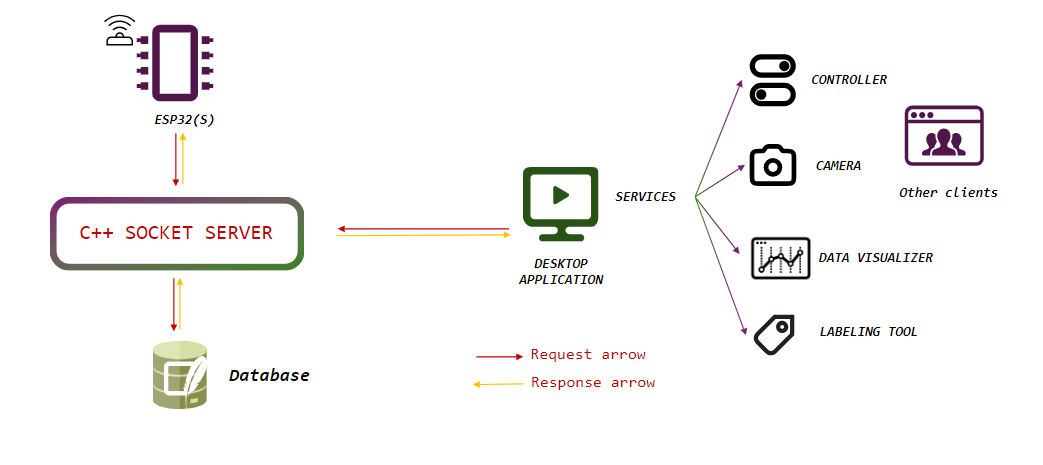
\includegraphics[width=12cm,height=5cm]{image/anh4.png}
    \caption{Mô hình cho hệ thống} \label{EV}
\end{figure}
\subsubsection{Phần mềm}
\textbf{Phần mềm}\\
\begin{itemize}
    \item Text editor: Visual Code. 
    \item Language: C++. 
    \item Database: SQLite database. 
    \item Build tool: CMake. 
    \item Source Control Systems: Git \& Github. 
\end{itemize}
\hspace{1cm}
\textbf{Desktop Application: }
\begin{itemize}
    \item Text editor: Visual Code
    \item Environment: Nodejs. 
    \item Language: TypeScript.
    \item Dependencies: ElectronJS, ReactJS, Tailwind CSS, Flowbite-React, …
\end{itemize}
\cleardoublepage
\section*{Chương 3.Kết quả đạt được}
\addcontentsline{toc}{section}{\numberline{}Chương 3.Kết quả đạt được}
\setcounter{section}{3}
\setcounter{subsection}{0}
Nguyên lý hoạt động của cảm biến vật cản hồng ngoại thụ động (PIR) dựa trên việc sử dụng một cặp cảm biến nhiệt điện để phát hiện năng lượng nhiệt từ sóng hồng ngoại trong môi trường xung quanh. Hai cảm biến này được đặt cạnh nhau và khi có sự chênh lệch về tín hiệu giữa chúng (ví dụ: khi một người di chuyển vào phòng), cảm biến hồng ngoại sẽ kích hoạt. Thiết bị có thể kích hoạt báo động, thông báo cho cơ quan chức năng (qua loa báo, đèn báo…) hoặc tự động bật/tắt đèn, quạt.

Bức xạ hồng ngoại được tập trung vào mỗi cảm biến nhiệt điện thông qua một loạt thấu kính Fresnel, được thiết kế như vỏ của cảm biến. Những thấu kính này mở rộng vùng cảm nhận của cảm biến, cho phép nó bao quát hầu hết khu vực xung quanh mắt cảm biến hồng ngoại. Thấu kính Fresnel giúp tối ưu hóa khả năng phát hiện, đảm bảo rằng ngay cả những chuyển động nhỏ cũng được ghi nhận, nâng cao hiệu quả và độ chính xác của cảm biến.
\begin{figure}[H]
    \centering
    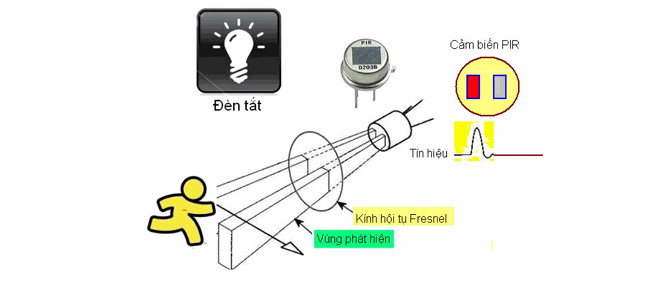
\includegraphics[width=12cm,height=5cm]{image/anh5.png}
    \caption{Mô hình cho hệ thống} \label{EV}
\end{figure}
\subsection{Phần cứng và vi điều khiển}
*Mạch cứng\\
Sơ đồ nguyên lý của mạch PIR bao gồm các thành phần chính như cảm biến PIR, bộ khuếch đại để tăng cường tín hiệu từ cảm biến, bộ lọc để loại bỏ các nhiễu không mong muốn và đảm bảo rằng chỉ các tín hiệu có ý nghĩa mới được xử lý, cùng với các linh kiện bổ sung khác như điện trở, tụ điện và vi điều khiển để đảm bảo toàn bộ hệ thống hoạt động ổn định và chính xác.
 
\begin{figure}[H]
    \centering
    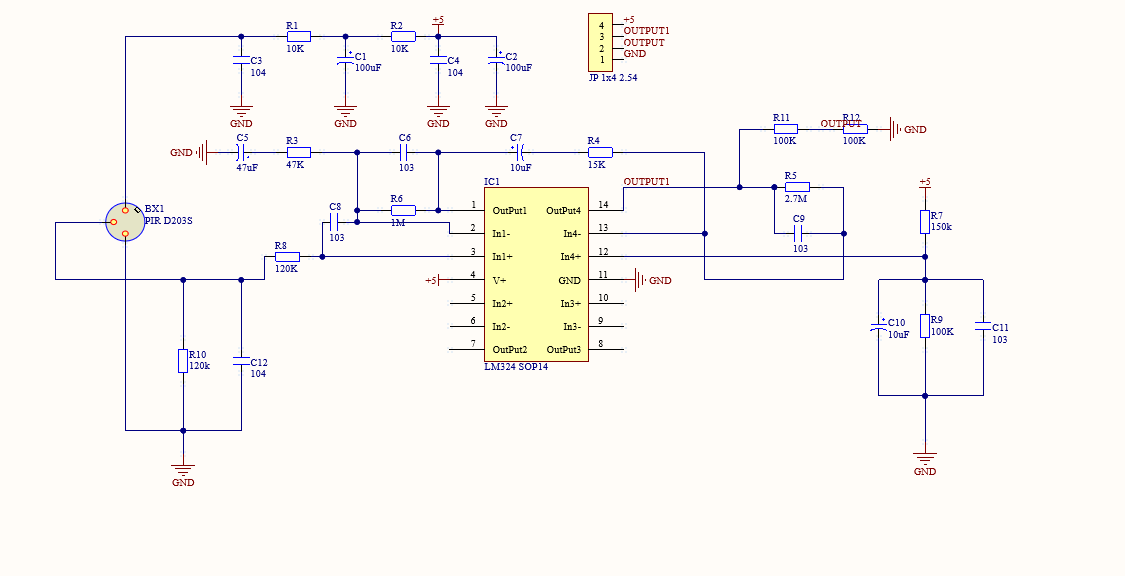
\includegraphics[width=10cm,height=5cm]{image/anh6.png}
    \caption{Mạch nguyên lý} \label{EV}
\end{figure}

\begin{figure}[H]
    \centering
    \begin{subfigure}[b]{0.45\textwidth}
        \centering
        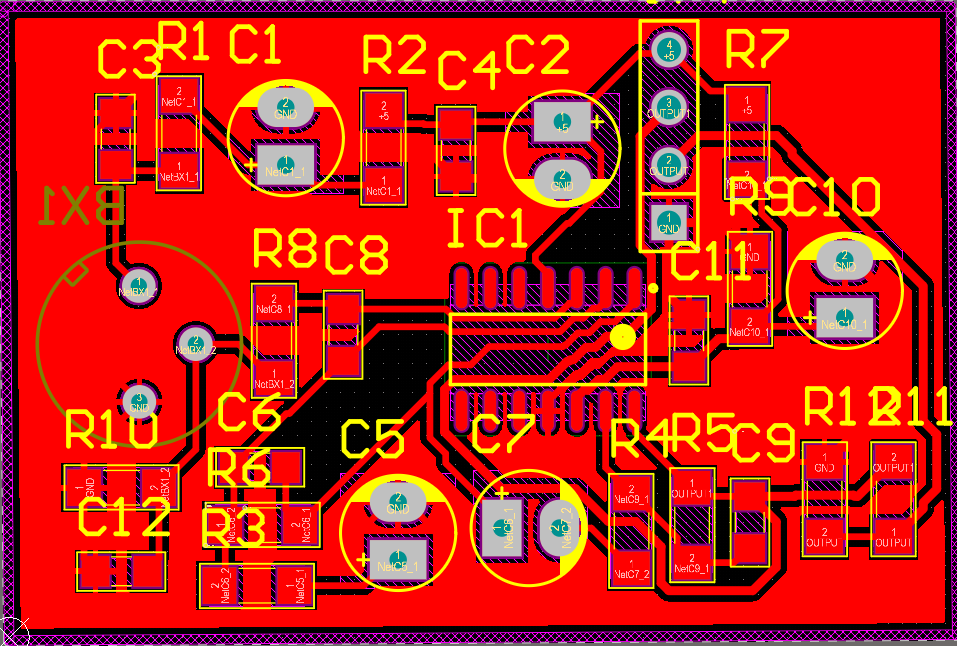
\includegraphics[width=\textwidth,height=5cm]{image/anh7.png}
        \caption{PCB} \label{EV1}
    \end{subfigure}
    \hfill
    \begin{subfigure}[b]{0.45\textwidth}
        \centering
        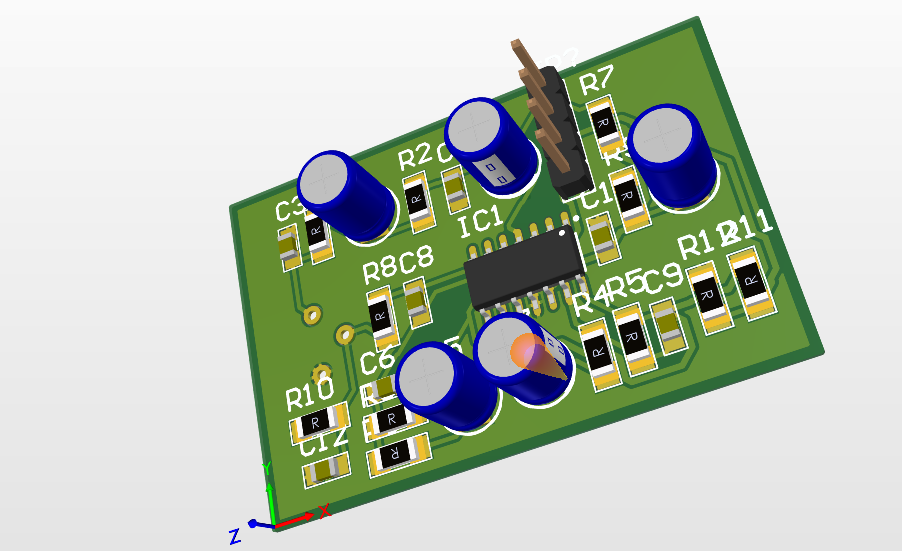
\includegraphics[width=\textwidth,height=5cm]{image/anh8.png}
        \caption{3D} \label{EV2}
    \end{subfigure}
    \caption{Mạch in 3D}
    \label{fig:two_graphs}
\end{figure}

\begin{figure}[H]
    \centering
    \begin{subfigure}[b]{0.45\textwidth}
        \centering
        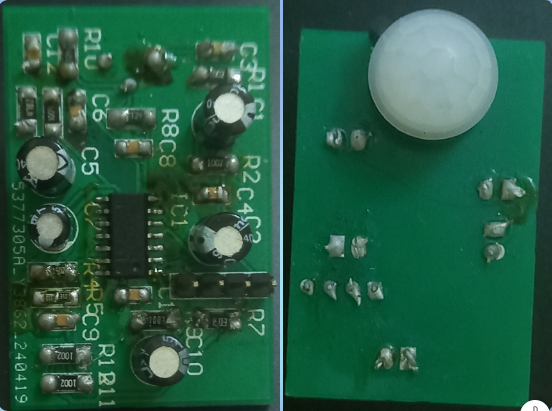
\includegraphics[width=6cm,height=6cm]{image/anh10.png}
        \caption{Mạch thật} \label{EV1}
    \end{subfigure}
    \hfill
    \begin{subfigure}[b]{0.45\textwidth}
        \centering
        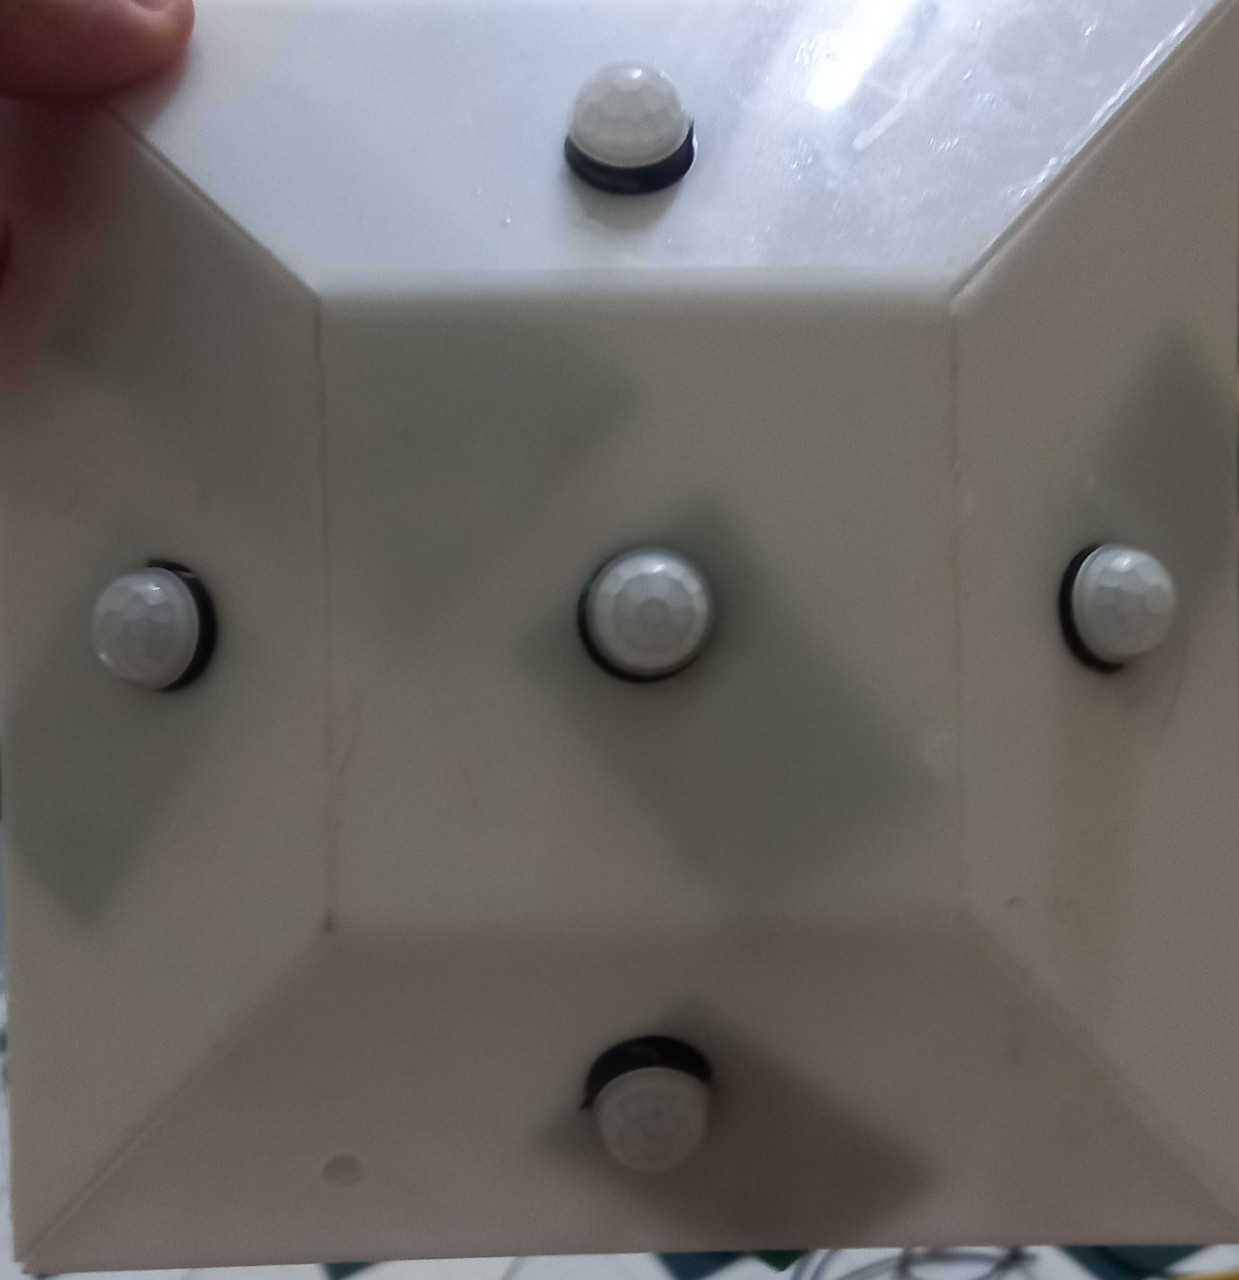
\includegraphics[width=6cm,height=6cm]{image/anh_pir.jpg}
        \caption{PIR ARRAY} \label{EV2}
    \end{subfigure}
    \caption{Sản phẩm}
    \label{fig:two_graphs}
\end{figure}
*Thu dữ liệu\\
\begin{itemize}
    \item[] \textbf{Sử dụng ESP32:}

    ESP32 được sử dụng làm vi điều khiển chính cho hệ thống. ESP32 có tích hợp Wi-Fi và Bluetooth, giúp dễ dàng thu thập và truyền dữ liệu từ cảm biến PIR đến các thiết bị khác hoặc server.
    
    \item[] \textbf{Môi trường phát triển ESP IDF:}

    ESP-IDF (Espressif IoT Development Framework) là môi trường phát triển chính thức của Espressif dành cho ESP32. Nó cung cấp các công cụ và thư viện cần thiết để phát triển ứng dụng trên ESP32.
    
    \item[] \textbf{Sử dụng FreeRTOS:}

    FreeRTOS là một hệ điều hành thời gian thực được sử dụng trên ESP32 để quản lý các tác vụ và tài nguyên của hệ thống. Nó giúp đảm bảo rằng các tác vụ xử lý dữ liệu từ cảm biến PIR và truyền thông với server được thực hiện một cách hiệu quả và đáng tin cậy.
\end{itemize}


\subsection{Phần mềm}
\textbf{-Phát triển HTTP\_Module xử lý HTTP:}

HTTP\_Module được phát triển để xử lý các yêu cầu HTTP, bao gồm gửi và nhận dữ liệu từ server. Module này đảm bảo rằng dữ liệu từ cảm biến PIR có thể được truyền tới server một cách an toàn và hiệu quả.

\textbf{-Hoàn thành xong Server với các API cơ bản:}

Server được triển khai với các API cơ bản để nhận, xử lý và lưu trữ dữ liệu từ các cảm biến PIR. Các API này cung cấp các chức năng cần thiết để giao tiếp với ESP32 và quản lý dữ liệu.
\begin{figure}[H]
    \centering
    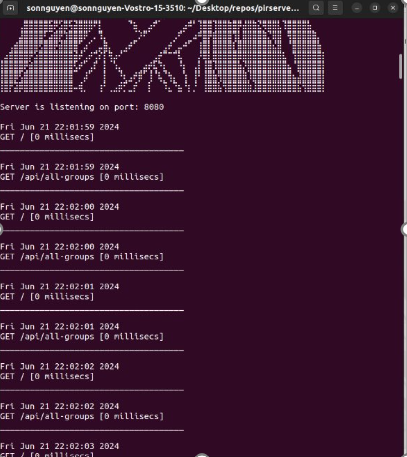
\includegraphics[width=6cm,height=8cm]{image/anh13.png}
    \caption{Server đang thu dữ liệu từ ESP32 gửi lên} \label{EV}
\end{figure}
\textbf{-Hoàn thành cơ chế quay, trực quan hóa dữ liệu và gán nhãn cho Desktop App:}


Desktop App được phát triển để trực quan hóa dữ liệu thu thập từ cảm biến PIR. App này cung cấp các chức năng như quay lại dữ liệu, hiển thị trực quan thông tin và gán nhãn dữ liệu để phân tích và theo dõi.

Nhóm đã hoàn thành các bước từ phát triển phần cứng, vi điều khiển, thu thập dữ liệu, cho đến phần mềm xử lý và trực quan hóa, tạo nên một hệ thống hoàn chỉnh và hiệu quả trong việc phát hiện và xử lý dữ liệu từ cảm biến PIR.
\begin{figure}[H]
    \centering
    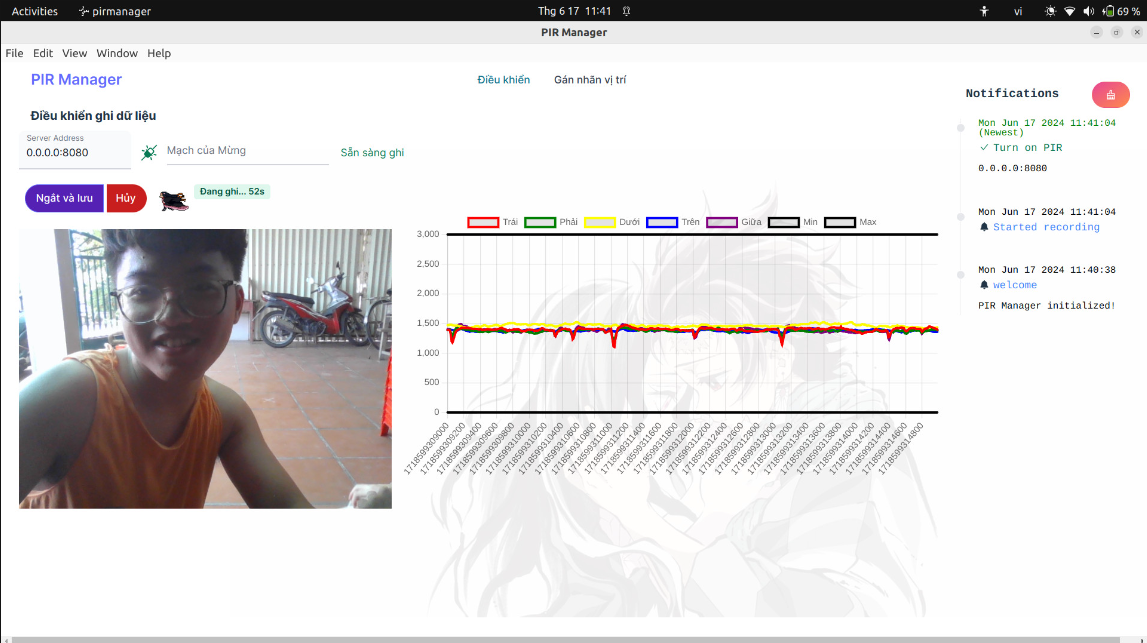
\includegraphics[width=12cm,height=7cm]{image/anh11.png}
    \caption{Giao diện app} \label{EV}
\end{figure}
\begin{figure}[H]
    \centering
    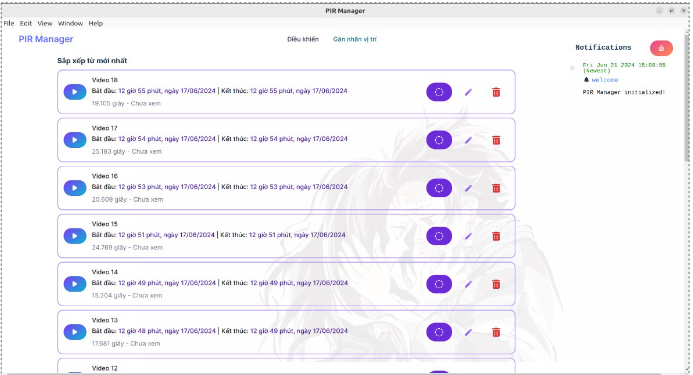
\includegraphics[width=12cm,height=7cm]{image/anh12.png}
    \caption{Chức năng gán nhãn phục vụ cho bên AI} \label{EV}
\end{figure}

\subsection{Thiết lập bối cảnh thu data}
\textbf{Thử nghiệm:}
\begin{itemize}
    \item Nguồn cấp cho vi điều khiển: chân USB
    \item Vị trí: ngoài trời
    \item Nhiệt độ: ~ 30 độ C
    \item Diện tích thử nghiệm: 3 x 3 m\(^2\)
\end{itemize}


\begin{figure}[H]
    \centering
    \begin{subfigure}[b]{0.45\textwidth}
        \centering
        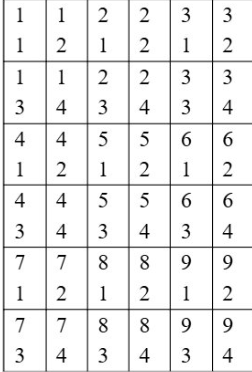
\includegraphics[width=5cm,height=7cm]{image/anh14.png}
        \caption{Chia thành các vùng nhỏ} \label{EV1}
    \end{subfigure}
    \hfill
    \begin{subfigure}[b]{0.45\textwidth}
        \centering
        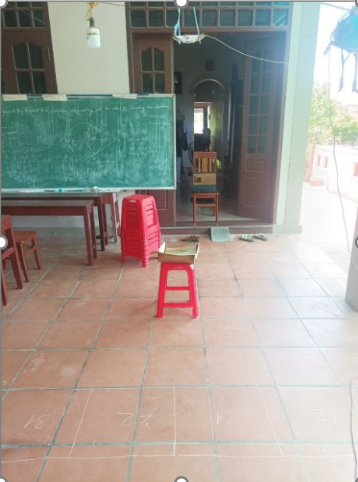
\includegraphics[width=5cm,height=7cm]{image/anh15.png}
        \caption{HIện trường} \label{EV2}
    \end{subfigure}
    \caption{Bối cảnh thu data}
    \label{fig:two_graphs}
\end{figure}
\textbf{Kết quả:}
\begin{figure}[H]
    \centering
    \begin{subfigure}[b]{0.45\textwidth}
        \centering
        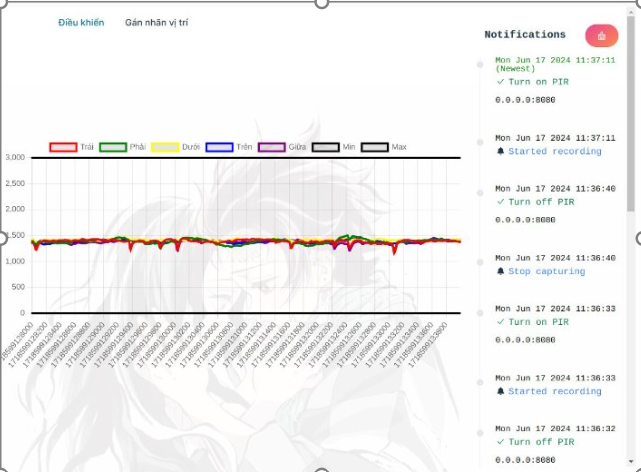
\includegraphics[width=8cm,height=6cm]{image/anh16.png}
        \caption{Dữ liệu khi không có chuyển động} \label{EV1}
    \end{subfigure}
    \hfill
    \begin{subfigure}[b]{0.45\textwidth}
        \centering
        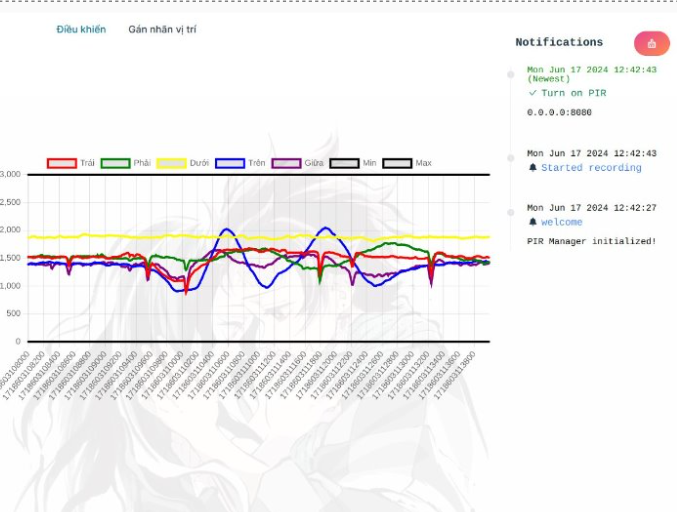
\includegraphics[width=8cm,height=6cm]{image/anh17.png}
        \caption{Đi từ ô 11 đến 32 (Hàng đầu tiên)} \label{EV2}
    \end{subfigure}
    \caption{Đồ thị thể hiện giá trị ADC các cảm biến}
    \label{fig:two_graphs}
\end{figure}

\begin{figure}[H]
    \centering
    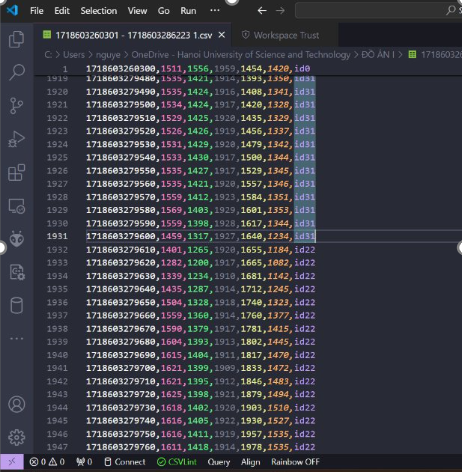
\includegraphics[width=7cm,height=10cm]{image/anh18.png}
    \caption{Một mẫu csv đầu ra, đã được gán nhãn.} \label{EV}
\end{figure}
\cleardoublepage
\section*{Chương 4.Vấn đề còn tồn đọng và khó khăn}
\addcontentsline{toc}{section}{\numberline{}Chương 4.Vấn đề còn tồn đọng và khó khăn}
\setcounter{section}{4}
\setcounter{subsection}{0}
\textbf{Nhiễu trong quá trình đọc ADC:}

Trong quá trình thực hành thử nghiệm phát hiện việc kết nối Wifi và mở cổng Socket có ảnh hưởng đến số ADC mà ESP32 đọc được. Cụ thể, tốc độ kết nối Wifi càng yếu, thời gian mở cổng Socket càng lâu thì điện áp đọc được càng bị kéo xuống thấp, thậm chí là về 0 trong 1 khoảng thời gian.

\begin{figure}[H]
    \centering
    \begin{subfigure}[b]{0.45\textwidth}
        \centering
        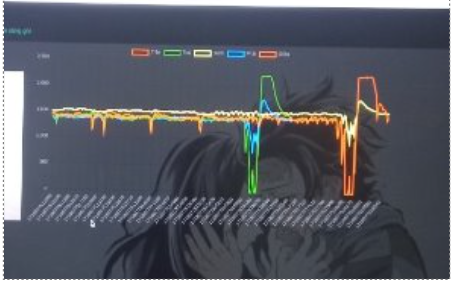
\includegraphics[width=8cm,height=6cm]{image/anh19.png}
        \caption{Dữ liệu kết nối kém} \label{EV1}
    \end{subfigure}
    \hfill
    \begin{subfigure}[b]{0.45\textwidth}
        \centering
        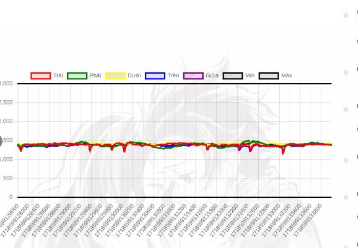
\includegraphics[width=8cm,height=6cm]{image/anh20.png}
        \caption{Dữ liệu kết nối tốt hơn} \label{EV2}
    \end{subfigure}
    \caption{Nhiễu trong quá trình đọc ADC}
    \label{fig:two_graphs}
\end{figure}
\textbf{Dự đoán về nguyên nhân:\\}

Dù chưa kịp có những thử nghiệm chi tiết, nhưng về mặt dự đoán, nhiễu lớn này gây ra có thể bởi một trong các lý do sau:
\begin{itemize}
    \item Việc sử dụng Wifi làm ảnh hưởng đến đầu đọc ADC hoặc phần hàm để lấy dữ liệu ADC.
    \item Việc sử dụng Wifi đã lấy mất phần năng lượng để cung cấp điện áp cho chân nguồn 3.3V, dẫn tới sụt nguồn cho toàn bộ 5 con PIR.
\end{itemize}
Trong đó, nguyên nhân thứ hai là nguyên nhân khả quan hơn.
\cleardoublepage
\section*{Chương 5:Kết luận chung và hướng phát triển}
\addcontentsline{toc}{section}{\numberline{}Chương 5:Kết luận chung và hướng phát triển}
\setcounter{section}{5}
\setcounter{subsection}{0}

\subsection{Tóm tắt nội dung nghiên cứu}
Trong bối cảnh cuộc cách mạng công nghiệp 4.0 đang diễn ra mạnh mẽ, việc ứng dụng các công nghệ cảm biến thông minh vào đời sống và sản xuất trở nên ngày càng cần thiết. Dự án "Mạch phần cứng và truyền thông RF cho hệ thống thu thập dữ liệu PIR" đã thành công trong việc thiết kế và triển khai một hệ thống hoàn chỉnh, bao gồm phần cứng, vi điều khiển, server và phần mềm quản lý.

Chúng tôi đã tiến hành thiết kế một mạch cứng với 5 cảm biến PIR, cho phép thu thập tín hiệu hồng ngoại từ môi trường xung quanh và chuyển đổi chúng thành giá trị số. Hệ thống vi điều khiển ESP32 được lập trình để đọc và truyền tải dữ liệu qua kết nối Wi-Fi đến một server được xây dựng bằng ngôn ngữ C++, lưu trữ trong cơ sở dữ liệu SQLite. Phần mềm quản lý trên desktop, phát triển bằng NodeJS, cung cấp giao diện người dùng để điều khiển, trực quan hóa và gán nhãn dữ liệu.
\subsection{ Ý nghĩa và ứng dụng thực tiễn}
Hệ thống thu thập dữ liệu PIR này không chỉ là một giải pháp kỹ thuật hoàn chỉnh mà còn mở ra nhiều cơ hội ứng dụng thực tiễn trong đời sống và công nghiệp:
\begin{itemize}
    \item Ứng dụng trong nhà thông minh (Smart Home): Hệ thống có thể được tích hợp vào các thiết bị và hệ thống nhà thông minh để phát hiện chuyển động, điều khiển ánh sáng, an ninh, và nhiều ứng dụng khác.
    \item Giám sát an ninh: Với khả năng phát hiện chuyển động chính xác, hệ thống có thể được sử dụng trong các hệ thống giám sát an ninh để phát hiện xâm nhập trái phép.


\end{itemize}
\subsection{Hướng phát triển trong tương lai}
Dù đã đạt được nhiều kết quả đáng khích lệ, dự án vẫn còn nhiều tiềm năng phát triển:
\begin{itemize}
    \item Nâng cao độ chính xác và khả năng nhận diện: Tích hợp các thuật toán học máy để phân tích dữ liệu từ cảm biến, giúp nâng cao độ chính xác và khả năng nhận diện các đối tượng và hành vi phức tạp hơn
    \item Mở rộng số lượng cảm biến: Tăng số lượng cảm biến trong mạch cứng để mở rộng phạm vi giám sát và thu thập dữ liệu.
    \item Tối ưu hóa hiệu suất: Cải thiện hiệu suất của vi điều khiển và server để xử lý dữ liệu nhanh hơn và tiết kiệm năng lượng hơn.
\end{itemize}
\subsection{Lời cảm ơn}
Chúng em xin chân thành cảm ơn PGS.TS Nguyễn Quốc Cường đã tận tình hướng dẫn và hỗ trợ chúng em trong suốt quá trình thực hiện đề tài này. Chúng em cũng xin cảm ơn các thầy cô và bạn bè đã luôn động viên và giúp đỡ chúng em hoàn thành dự án này. Dự án không chỉ là kết quả của những nỗ lực cá nhân mà còn là sự hợp tác và hỗ trợ từ nhiều phía.

Dự án "Mạch phần cứng và truyền thông RF cho hệ thống thu thập dữ liệu PIR" đã mang lại cho chúng em nhiều kiến thức và kinh nghiệm quý báu, giúp chúng em hiểu sâu hơn về công nghệ cảm biến và hệ thống nhúng, mở ra nhiều cơ hội cho các nghiên cứu và ứng dụng trong tương lai.
\cleardoublepage

\begin{thebibliography}{99}

    \bibitem{DB203B}
    DB203B Datasheet
    
    \bibitem{Ngamakeura2021}
    K. Ngamakeura, S. Yongchareon, J. Yu, and S. Islam, ``Passive infrared sensor dataset and deep learning models for device-free indoor localization and tracking,'' \textit{Journal/Conference Name}, 2021.
    
    \bibitem{Wu2021}
    L. Wu and Y. Wang, ``Stationary and moving occupancy detection using the SLEEPIR sensor module and machine learning,'' \textit{Journal/Conference Name}, 2021.
    
    \end{thebibliography}
    
    
\end{document}
